% CVPR 2027 draft v0 (2026-10-25).
% Numbers: ../../results (vlm/FINDINGS.md, ext/SUMMARY_atty.md, robust_all.json). Figures: ../../analysis/fig_*.py.
% Red \pend{} = result still running or to verify. Blue \note{} = comment for the authors, delete before submission.
\documentclass[10pt,twocolumn,letterpaper]{article}
\usepackage[review]{cvpr}
\usepackage{graphicx,booktabs,amsmath,amssymb,amsthm,multirow,xcolor}
\usepackage{caption}
\definecolor{cvprblue}{rgb}{0.21,0.49,0.74}
\usepackage[pagebackref,breaklinks,colorlinks,allcolors=cvprblue]{hyperref}
\newcommand{\pend}[1]{{\color{red}[#1]}}
\newcommand{\note}[1]{{\color{blue}[Note: #1]}}
\newcommand{\pmsd}[1]{{\scriptsize$\pm$#1}}
\newtheorem{proposition}{Proposition}
\def\paperID{*****}\def\confName{CVPR}\def\confYear{2027}
\title{Whoever Picks the Evidence Decides:\\Selection Attacks on High-Resolution Vision and a Redundant Presenter}
\author{Anonymous CVPR submission}
\begin{document}
\maketitle

%=====================================================================
\begin{abstract}
High-resolution vision models rarely look at their whole input. A zoom tool, a crop selector or a cheap tile scorer decides which regions the expensive model inspects. We show that this selection step is an attack surface that no pixel-level defence covers. An attacker who controls only the selector, and shows nothing but real, unmodified regions of the image, controls the answer. On V$^*$ and HR-Bench, choosing which crops a Qwen2.5-VL or Qwen3-VL judge sees lowers accuracy from .69--.91 to .34--.39. In whole-slide pathology, a compromised tile selector drives an efficient multiple-instance learning pipeline to chance or below on CAMELYON17, TCGA-RCC and TCGA-NSCLC. The RL-trained zoom agent that actually uses its crops (Mini-o3) is steered to a committed wrong answer on 30\% of the questions it answers correctly. We then ask how to present evidence so that no single selection component decides. One advocate per hypothesis is not enough: an attacker who takes the true answer's advocate is as harmful as one who takes a single selector. A \emph{hybrid presenter}, made of per-hypothesis advocates plus one label-free neutral slot, tolerates the compromise of any one component. Against a judge-aware adaptive attacker it keeps .59--.71 accuracy on natural images (+.20 to +.37 over the compromised single selector; all paired 95\% CIs exclude zero) and .67--.71 on pathology (vs.\ $\le$.02). Clean accuracy is unchanged in five of six settings.
\end{abstract}

%=====================================================================
\section{Introduction}\label{sec:intro}
\note{opening paragraph: one concrete scene. A radiology/pathology AI that only reads the regions a triage model hands it; or a VLM agent that answers from the crop its zoom tool returns. The person who controls that hand-off controls the answer, and nothing in the output looks wrong.}

A 4K photograph or a $10^5$-tile whole-slide image (WSI) is too large to process at full resolution, so high-resolution vision pipelines \emph{select}. Base vision-language models (VLMs) answer from a low-resolution overview plus a few zoomed crops~\cite{wu2024vstar,zhang2025vicrop}. RL-trained ``thinking-with-images'' agents call a zoom tool themselves~\cite{zheng2025deepeyes,pixelreasoner,minio3}. Efficient WSI classifiers let a cheap low-magnification network pick the few tiles that a pathology foundation model encodes~\cite{admil2026,eagle2026}. In each case one component decides what the expensive model sees.

We study what happens when that component is not trustworthy, because it is buggy, swapped, or controlled by an adversary. Our attacker is deliberately weak in what it may \emph{show}: it never perturbs a pixel and never injects text. It may only choose which real regions of the input are presented, under the same budget as the honest selector. Pixel-level adversarial defences~\cite{foote2021now,mil_adv2022} and prompt-injection defences~\cite{wu2024agentattack,crossinject2025} do not apply, because every presented region is genuine.

\textbf{Selection is an attack surface} (Sec.~\ref{sec:attack}). With the overview always visible, choosing the crops lowers Qwen2.5-VL from .81 to .37 on V$^*$ and from .69 to .39 on HR-Bench-4K, and Qwen3-VL from .91 to .34. In pathology, the same attack sends an efficient single-selector pipeline to $\kappa=-.24$ on CAMELYON17 and to .02/.00 balanced accuracy on TCGA-RCC/NSCLC, i.e.\ to the attacker's class on nearly every slide. Concurrent work shows that some RL zoom agents ignore their crops~\cite{wang2026illusion,liu2025faithful}. We confirm this and show the flip side: those agents are immune only because their zoom adds nothing, while the agent whose zoom carries information (Mini-o3) can be hijacked.

\textbf{Redundant presentation} (Sec.~\ref{sec:method}). Debate~\cite{irving2018debate,khan2024debate} suggests giving every hypothesis its own advocate, so a compromised selector can no longer hide the evidence for the truth. We find that this is not enough. If the attacker takes the \emph{true} answer's advocate, the judge sees only evidence for wrong answers and accuracy falls to the compromised-single-selector level (.27--.43 on natural images; .15--.59 in pathology). Adding one label-free neutral slot fixes this. Under any single compromise, either the true advocate or the neutral slot stays honest (Prop.~\ref{prop:cover}). This \emph{hybrid presenter} needs no knowledge of which component is compromised and adds one slot of cost.

\textbf{Contributions.}
\textbf{(1)} A threat model and attacks for evidence selection in high-resolution vision that use only real, unmodified regions, evaluated in two domains (natural-image VLMs, gigapixel pathology), and on RL zoom agents.
\textbf{(2)} The finding that per-hypothesis advocates fail when the true advocate is compromised, and a hybrid presenter with a simple coverage guarantee that tolerates any single compromised component.
\textbf{(3)} An evaluation against judge-aware adaptive attackers in six settings (3 seeds $\times$ 5 folds in pathology, paired bootstrap CIs on natural images), showing that the fragility is adversarial-only: a weak but honest selector costs $\le$.01.

\begin{figure*}[t]\centering
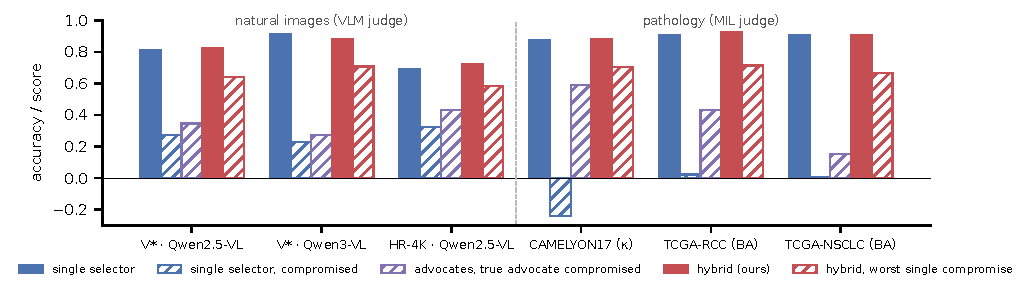
\includegraphics[width=\textwidth]{../figs/fig_robust_all.pdf}
\caption{\textbf{Whoever picks the evidence decides, unless no single picker does.} Accuracy (natural images; letter scoring) or $\kappa$ / balanced accuracy (pathology) for a single selector (blue), per-hypothesis advocates (purple) and the hybrid presenter (red), honest (solid) and with one component compromised (hatched). Hybrid, compromised = worst case per question/slide over which component the attacker takes, using a judge-aware adaptive attacker. \pend{single selector, compromised: switches to the judge-aware attacker when the matched runs finish (jobs 7299072/85/90)}}\label{fig:main}
\end{figure*}

%=====================================================================
\section{Related work}\label{sec:related}
\textbf{Zooming in high-resolution vision.} V$^*$~\cite{wu2024vstar} and HR-Bench~\cite{hrbench} show that MLLMs miss small details in large images. Training-free crop selection~\cite{zhang2025vicrop,hrbench} and RL-trained zoom agents~\cite{zheng2025deepeyes,pixelreasoner,minio3} recover them. Several 2025--26 papers ask whether these agents actually use what they zoom on. Liu \etal~\cite{liu2025faithful} corrupt the visual part of the reasoning chain, and Wang \etal~\cite{wang2026illusion} replace returned crops with random or blank ones and find that DeepEyes-style agents barely change their answers while Mini-o3 collapses. We use the same crop-substitution protocol as a starting point (Sec.~\ref{sec:agents}). Our question is different: not whether the crops matter, but what an adversary can do when they do, and how to present evidence so that no single selector decides. Evidence-grounding benchmarks~\cite{viebench2026,pixeleyes2026,med2026} and distractor robustness~\cite{distract2026} are complementary.

\textbf{Efficient whole-slide inference.} MIL on foundation-model features~\cite{ilse2018abmil,lu2021data,uni,conch} reads every tile. ZoomMIL~\cite{thandiackal2022zoommil}, RLogist~\cite{zhao2023rlogist}, ADMIL~\cite{admil2026} and EAGLE~\cite{eagle2026} select a few tiles with a cheap model first. Recent work measures how selection changes the evidence MIL sees~\cite{bagshift2026,foci2026} and regularises attention to be faithful~\cite{gcemil2026,carmil2026}. None of these considers a compromised selector.

\textbf{Adversarial robustness.} Attacks on MIL perturb tile pixels or features~\cite{foote2021now,mil_adv2022}. Attacks on multimodal agents perturb images or inject instructions~\cite{wu2024agentattack,crossinject2025}. Our attacker does neither; it chooses which authentic regions to show.

\textbf{Debate and prover--verifier games.} Debate~\cite{irving2018debate,khan2024debate,kenton2024scalable}, prover--verifier games~\cite{anil2021pvg,kirchner2024pvg} and Merlin--Arthur classifiers~\cite{waldchen2024merlin} let untrusted provers present evidence to a weaker verifier. Merlin--Arthur in particular pairs a cooperative and an adversarial feature selector. Our advocates follow this idea. Our finding that they fail when the true side's prover is compromised, and our neutral-slot fix, apply to that setting as well.

%=====================================================================
\section{Threat model}\label{sec:threat}
An input $x$ (image or slide) is split into candidate regions $\mathcal{R}(x)=\{r_1,\dots,r_N\}$: grid crops of a photograph, or tiles of a slide. A \emph{presenter} is a set of slots $s=1..m$. Each slot is filled by a selection rule $\sigma_s$ that returns at most $B_s$ regions, optionally with a text label (\eg ``evidence for option (B)''). The judge $J$ sees the presentation $P(x)=\{(\sigma_s(x),\ell_s)\}_s$, plus a global low-resolution overview for natural images, and outputs a class.

\textbf{Attacker.} The attacker compromises \emph{one} slot $s$ of its choice and replaces $\sigma_s$ by any rule that returns at most $B_s$ regions from $\mathcal{R}(x)$; it cannot change the labels, the other slots, or the pixels. It knows the true label (the strongest case for an attacker that wants a wrong answer) and has white-box access to the scores of the judge. We use three strengths:
(i) \emph{fixed}: show the regions that most favour the strongest wrong class, scored by the judge on each region alone;
(ii) \emph{per-region white-box}: the same with scores computed under the compromised slot's label;
(iii) \emph{judge-aware adaptive}: search over candidate regions to minimise the judge's probability of the true class \emph{on the full presentation}, including the honest slots. In pathology it greedily builds the set (top-128 candidates); on natural images it tries the top-8 tiles per slot.
The worst case is taken per input over every slot the attacker may take. That includes the true class's advocate and the neutral slot.

%=====================================================================
\section{Presenters}\label{sec:method}
\textbf{Single selector.} One slot: the $B$ regions the judge (natural images) or the distilled cheap scorer (pathology, ADMIL-style~\cite{admil2026}) finds most informative, unlabelled.

\textbf{Advocates.} One slot per hypothesis $c\in\{1..C\}$. Advocate $c$ shows the regions that best support $c$ under the cheap scores and is labelled ``evidence presented to support option ($c$)''. On natural images this is the tile with the highest score for $c$; in pathology it is the top-$K_c$ tiles by margin for $c$, with structure-aware rules for metastasis stages (supplement). No label is used at test time.

\textbf{Hybrid presenter.} The advocates plus one \emph{neutral} slot that shows the single selector's choice without a label (``Zoomed-in view'' on natural images; a separate slot flag in pathology).

\textbf{Judge.} On natural images the judge is the frozen VLM; we score the option letters directly. In pathology the judge is a gated-attention MIL model over the presented tiles, each tagged with a one-hot slot flag. It is trained on honest presentations and on presentations with one slot replaced by the white-box attacker, for three rounds, over every (slot, target class) pair the attacker may use (supplement).

\textbf{Why the neutral slot.} The following is the design principle behind the hybrid. It is elementary, but it explains why advocates alone fail and what property of the judge the hybrid relies on.
Call an honest slot a \emph{witness} for input $(x,y)$ if it is the advocate of $y$ or the neutral slot. Say the judge is \emph{witness-sufficient} on $(x,y)$ if $J$ predicts $y$ on every presentation that contains at least one honest witness, whatever the other slots show.
\begin{proposition}\label{prop:cover}
If $J$ is witness-sufficient on $(x,y)$, the hybrid presenter is correct on $(x,y)$ under the compromise of any single slot. No such guarantee exists for the single selector or for pure advocates. For the single selector, a compromise leaves no honest slot. For advocates, compromising the advocate of $y$ leaves no witness, and the remaining honest slots only argue for wrong classes.
\end{proposition}
\begin{proof}
The hybrid has two witnesses, the advocate of $y$ and the neutral slot. One compromise removes at most one of them.
\end{proof}
Witness-sufficiency is a property of the judge, not of the presenter, and we do not assume it. We measure it. Every input that the attacker flips under the hybrid is one on which the judge is not witness-sufficient, so the drop from honest to worst case (Tab.~\ref{tab:vlm}) lower-bounds how often witness-sufficiency fails. Adversarial training of the judge in pathology is meant to increase witness-sufficiency. Training-free, the VLM judge already has it on most inputs.

\textbf{Cost.} The hybrid encodes the advocates' regions plus the neutral slot. On natural images that is $C{+}1$ crops vs.\ $C$ for the single selector. In pathology the hybrid-$K$ variant doubles the tiles sent to the foundation model (2$K$ vs.\ $K$; 16--32 of 2--5K tiles). Encoding presented tiles takes $<$0.3\,s of a 5.5--7.9\,s selective pipeline, which is dominated by reading the slide at low magnification. Hybrid-$K_c$ adds only $K_c$ tiles and is reported too. \pend{clean single selector at budget 2$K$, for a matched-budget clean comparison}

%=====================================================================
\section{Experimental setup}\label{sec:setup}
\textbf{Natural images.} V$^*$-Bench~\cite{wu2024vstar} (191 questions, 2--4 options) and HR-Bench-4K~\cite{hrbench} (200 questions, 4 options; one rotation per question). Judges: Qwen2.5-VL-7B~\cite{qwen25vl} and Qwen3-VL-8B~\cite{qwen3vl}, frozen, scored by the log-probability of each option letter. The overview is resized to 768$^2$ pixels, and crops come from a two-scale grid (side $1/4$ and $1/2$ of the short image side, 50\% overlap) resized to 448$^2$ pixels. Per-tile scores $S\in\mathbb{R}^{N\times C}$ (overview + one tile) are cached and drive every selector and the fixed attacker. 95\% CIs: paired bootstrap over questions.

\textbf{Pathology.} CAMELYON17~\cite{camelyon17} (500 lymph-node slides, 4 stages, leave-one-hospital-out; quadratic-weighted $\kappa$), TCGA-RCC (882 slides, 3 subtypes) and TCGA-NSCLC (1{,}041 slides, 2 subtypes)~\cite{tcga} (5-fold patient-level CV; balanced accuracy). Cheap view: ImageNet EfficientNet-B0~\cite{tan2019efficientnet} at low magnification, with a 2-layer MLP distilled from a full-slide UNI/CONCH~\cite{uni,conch} ABMIL teacher. Budget $K=C\cdot K_c$ with $K_c=4$ (16/12/8 tiles). We report the mean over 5 folds, then the mean $\pm$ sd over 3 seeds.

\textbf{RL zoom agents.} DeepEyes-7B~\cite{zheng2025deepeyes}, PixelReasoner-RL-7B~\cite{pixelreasoner} and Mini-o3-7B~\cite{minio3} with their own prompts and tools, on V$^*$ and HR-Bench-4K. The overview is 768$^2$; we use full resolution for PixelReasoner as a check. Every tool call returns a substituted crop (Sec.~\ref{sec:agents}).

%=====================================================================
\section{Results}\label{sec:results}
\subsection{Selection is an attack surface}\label{sec:attack}
\begin{table}[t]\centering
\caption{\textbf{Natural images}, accuracy (95\% CI). Single = $C$ unlabelled crops; advocates = one labelled crop per option; hybrid = advocates + one neutral crop. ``Adaptive'': judge-aware attacker (top-8 tiles per slot). Hybrid worst = correct only if correct whichever component is compromised.}\label{tab:vlm}
\setlength{\tabcolsep}{3pt}\small
\begin{tabular}{@{}lccc@{}}\toprule
 & V$^*$ Q2.5 & V$^*$ Q3 & HR-4K Q2.5\\\midrule
overview only & .665 & .691 & \pend{} \\
single, honest & .812 & .911 & .690\\
single, compromised (fixed) & .366 & .335 & .390\\
single, compromised (adaptive) & \pend{} & \pend{} & \pend{}\\\midrule
advocates, honest & .806 & .843 & .705\\
\quad true advocate silenced & .419 & .387 & .475\\
\quad true advocate compromised (fixed) & .408 & .408 & .460\\
\quad true advocate compromised (adaptive) & .346 & .272 & .430\\\midrule
\textbf{hybrid}, honest & \textbf{.822} & .880 & \textbf{.720}\\
\quad true advocate compromised (adaptive) & .717 & .806 & .645\\
\quad neutral slot compromised (adaptive) & .670 & .728 & .610\\
\quad \textbf{worst case (adaptive)} & \textbf{.639} & \textbf{.707} & \textbf{.585}\\
 & {\scriptsize[.57,.71]} & {\scriptsize[.64,.77]} & {\scriptsize[.52,.66]}\\
hybrid worst $-$ single comp. & +.27 & +.37 & +.20\\
 & {\scriptsize[+.20,+.34]} & {\scriptsize[+.29,+.45]} & {\scriptsize[+.14,+.26]}\\\bottomrule
\end{tabular}\end{table}

\textbf{Natural images.} The right crops matter. On V$^*$ the overview alone gives .665 (Qwen2.5-VL), one crop of the ground-truth region raises it to .838, and a random crop gives .644. Because crops matter, choosing them is powerful. With the overview always visible, the compromised selector lowers accuracy to .37/.34/.39 (Tab.~\ref{tab:vlm}), well below the overview alone. The judge does not ignore misleading zoomed evidence. It defers to it.

\textbf{Pathology.} Efficient WSI pipelines depend even more on their selector, since the foundation model sees nothing else. The ADMIL-style single selector matches full-slide MIL within 1.4--2.6 points while encoding $<$1\% of tiles. When compromised it predicts the attacker's class on almost every slide (Tab.~\ref{tab:wsi}): $\kappa=-.24$ on CAMELYON17 and .02/.00 balanced accuracy on RCC/NSCLC, in every fold and seed.

\textbf{The fragility is adversarial-only.} A weak but honest selector, with the cheap scorer distilled from 10\% of the training slides, costs the single selector $\le$.01 (Tab.~\ref{tab:wsi}). The single selector is a fine estimator and a poor security boundary.

\begin{table}[t]\centering
\caption{\textbf{Pathology}, $\kappa$ (CAMELYON17) or balanced accuracy (TCGA); mean\pmsd{sd} over 3 seeds (each the mean of 5 folds). The attacker may take any slot, including the true class's advocate and the neutral slot; the judge is trained against all of these.}\label{tab:wsi}
\setlength{\tabcolsep}{2.5pt}\small
\begin{tabular}{@{}lccc@{}}\toprule
 & C17 $\kappa$ & RCC BA & NSCLC BA\\\midrule
single, honest & .873\pmsd{.026} & .907\pmsd{.023} & .909\pmsd{.008}\\
single, weak scorer (10\% data) & .867\pmsd{.030} & .899\pmsd{.013} & .901\pmsd{.003}\\
single, compromised & $-$.241\pmsd{.011} & .022\pmsd{.002} & .003\pmsd{.001}\\\midrule
advocates, honest & .823\pmsd{.015} & .920\pmsd{.010} & .874\pmsd{.007}\\
\quad per-tile attack & .685\pmsd{.017} & .670\pmsd{.001} & .530\pmsd{.023}\\
\quad adaptive attack & .589\pmsd{.029} & .433\pmsd{.004} & .153\pmsd{.004}\\
indep.\ scorers, attacked & .677\pmsd{.023} & .675\pmsd{.036} & .505\pmsd{.058}\\\midrule
hybrid-$K_c$, honest & .854\pmsd{.005} & .933\pmsd{.016} & .898\pmsd{.004}\\
\quad adaptive attack & .658\pmsd{.011} & .661\pmsd{.033} & .618\pmsd{.009}\\
\textbf{hybrid-$K$}, honest & \textbf{.879}\pmsd{.014} & \textbf{.924}\pmsd{.013} & .905\pmsd{.001}\\
\quad per-tile attack & .730\pmsd{.026} & .829\pmsd{.010} & .783\pmsd{.010}\\
\quad \textbf{adaptive attack} & \textbf{.705}\pmsd{.025} & \textbf{.713}\pmsd{.031} & \textbf{.665}\pmsd{.022}\\\bottomrule
\end{tabular}\end{table}

\subsection{Advocates are not enough; the hybrid is}\label{sec:hybrid}
\textbf{Advocates fail at the true advocate.} Honest advocates are as accurate as the single selector on V$^*$ with Qwen2.5-VL and on HR-Bench (.806, .705), and lower with Qwen3-VL (.843 vs.\ .911). When the attacker silences the advocate of the true option, accuracy drops to .39--.48. When it makes that advocate show the attacker's tile, accuracy drops to .27--.43 with the adaptive attacker, no better than a compromised single selector. In pathology the same holds once the attacker may take the true class's slot: .59/.43/.15 (Tab.~\ref{tab:wsi}). Independent cheap scorers for each advocate, which an attacker would have to compromise separately, do not help against this attacker either (.68/.68/.51). Diversity of selectors is not what matters. What matters is that some honest slot is not committed to a wrong class.

\textbf{The hybrid tolerates any single compromise.} Adding one neutral slot raises the per-input worst case to .64/.71/.59 on natural images (+.20 to +.37 over the compromised single selector; every paired CI excludes 0) and to .71/.71/.67 in pathology (vs.\ $-$.24/.02/.00). On natural images the neutral slot is the more attractive target in all three settings: the advocate of $y$ alone protects the judge more than the neutral slot does. The two slots fail on different inputs, though, so the per-input worst case is below either.

\textbf{Clean accuracy.} The honest hybrid matches or beats the honest single selector in five of six settings (.822 vs.\ .812, .720 vs.\ .690; .879/.924/.905 vs.\ .873/.907/.909). The exception is Qwen3-VL on V$^*$ (.880 vs.\ .911).

\textbf{Adaptive attacks.} A judge-aware attacker costs the hybrid another .06--.07 on natural images than the fixed attacker, and .03--.12 in pathology than the per-tile attacker. In pathology, the greedy set attacker is consistently stronger than the per-tile one (hybrid-$K$: .73$\to$.71, .83$\to$.71, .78$\to$.67), so we report it as the worst case. \pend{matched adaptive attacker for the single selector: if it lowers the single selector further, the gaps in Tab.~\ref{tab:vlm} grow}

\subsection{What about RL zoom agents?}\label{sec:agents}
\begin{table}[t]\centering
\caption{\textbf{RL zoom agents under crop substitution} (V$^*$, 768$^2$ overview): every zoom call returns the substituted crop. ``Confirms'': the answer text claims the zoom confirms the answer although the crop is blank. Mini-o3 rows: white-box attack (tiles chosen with Mini-o3's own option scores).}\label{tab:agents}
\setlength{\tabcolsep}{2.2pt}\small
\begin{tabular}{@{}lccccc@{}}\toprule
 & native & GT & random & blank & ``confirms''\\
 & & crop & crop & crop & on blank\\\midrule
DeepEyes & .681 & .717 & .694 & .691 & 90\%\\
PixelReasoner & .712 & .733 & .657 & .665 & 18\%\\
Mini-o3 & .848 & .743 & .228 & .178 & 2\%\\\midrule
\multicolumn{6}{@{}l}{Mini-o3, every zoom returns: \quad correct / committed wrong / abstains}\\
\quad GT crop & \multicolumn{5}{l}{.750 / .131 / .119}\\
\quad white-box adversarial & \multicolumn{5}{l}{.244 / .196 / .560}\\
\multicolumn{6}{@{}l}{hijacked (natively correct $\to$ committed wrong): 17\% (1 tile), 30\% (any of 4)}\\\bottomrule
\end{tabular}\end{table}

Concurrent work finds that some RL zoom agents ignore what their zoom returns~\cite{wang2026illusion,liu2025faithful}. We reproduce this with the same intervention (Tab.~\ref{tab:agents}). DeepEyes answers a blank grey crop as well as the right one (.691 vs.\ .717; HR-Bench: a .065 drop, CI [.03,.105]), and in 90\% of those answers it states that the zoom confirms the answer. Such an agent is immune to selection attacks only because its zoom carries no information. Mini-o3 is the opposite. Its zoom matters (.848$\to$.178 with blank crops; HR-Bench .70$\to$.18). When its zoom tool returns white-box adversarial tiles, it commits to a wrong answer on 30\% of the questions it natively answers correctly, and abstains on most of the rest. So under attack its accuracy falls to about .24, close to the compromised base VLM.

In other words, among the agents we test, a zoom is either decorative (and safe) or informative (and hijackable). This motivates evaluating presenters, not only agents, against selection attacks. \pend{optional: hybrid wrapper around Mini-o3 (Killarney)}

%=====================================================================
\section{Limitations}\label{sec:limits}
\textbf{One compromised component.} The guarantee and the experiments cover one compromised slot. Two colluding slots (the advocate of $y$ and the neutral slot) defeat the hybrid, as expected from Prop.~\ref{prop:cover}.
\textbf{The hybrid is degraded, not robust.} The worst case is .14--.24 below clean accuracy. The hybrid prevents collapse but does not remove the attack.
\textbf{Budget.} The hybrid shows one extra slot. In pathology hybrid-$K$ encodes 2$K$ tiles; the extra encoding time is small, but a matched-budget clean comparison is \pend{pending}.
\textbf{Label-aware attacker.} Our attacker knows the true label. This is the right worst case, but a realistic attacker targeting one wrong class without the label would be weaker.
\textbf{Scope.} Natural images use training-free VLM judges and letter scoring; we did not train a VLM judge against the attacker.

%=====================================================================
\section{Conclusion}
In high-resolution vision the component that picks the evidence is a single point of failure, even when every pixel it shows is real. Advocates for each hypothesis are the natural fix, but they fail exactly where it matters: at the true answer's advocate. One extra neutral slot is enough to prevent any single compromised component from deciding the answer, across natural-image VLMs and gigapixel pathology, at little cost in clean accuracy.

{\small
\bibliographystyle{ieeenat_fullname}
\bibliography{refs}}
\end{document}
